\documentclass[border=10pt]{standalone}
\usepackage{pgfplots}
\pgfplotsset{compat=1.18}
\usepgfplotslibrary{fillbetween}
\begin{document}
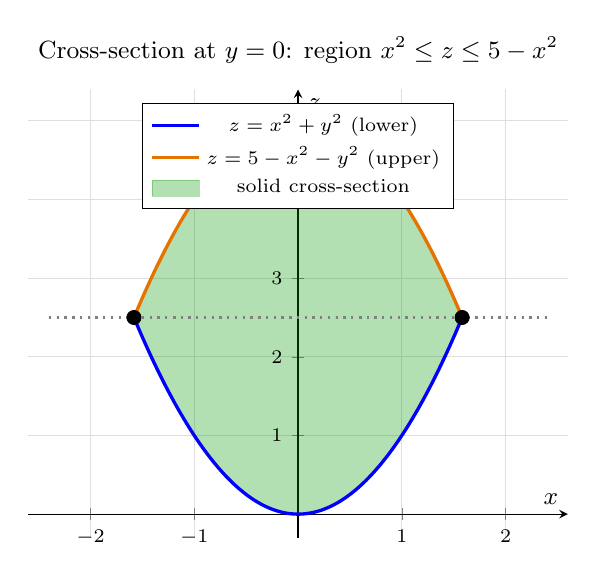
\begin{tikzpicture}
\begin{axis}[
    xlabel={$x$}, ylabel={$z$},
    xmin=-2.6, xmax=2.6, ymin=-0.3, ymax=5.4,
    axis lines=middle,
    grid=both,
    grid style={gray!25},
    title={Cross-section at $y=0$: region $x^2 \leq z \leq 5-x^2$},
    tick label style={font=\scriptsize},
    label style={font=\small},
    title style={font=\small},
    legend style={font=\scriptsize, at={(0.5,0.97)}, anchor=north},
    domain=-1.5811:1.5811, samples=100,
]
% Boundary curves with names
\addplot[name path=lower, blue, very thick] (x, {x^2});
\addplot[name path=upper, orange!90!black, very thick] (x, {5-x^2});
% Fill between the curves
\addplot[green!60!black, opacity=0.3] fill between[of=lower and upper];
% Intersection points
\addplot[only marks, mark=*, mark size=2.5pt, black]
    coordinates {(-1.5811, 2.5) (1.5811, 2.5)};
% Dashed line z = 5/2
\addplot[gray, dotted, thick, domain=-2.4:2.4] (x, {2.5});
\legend{$z=x^2+y^2$ (lower), $z=5-x^2-y^2$ (upper), solid cross-section}
\end{axis}
\end{tikzpicture}
\end{document}
